\documentclass[14pt]{extarticle}
\usepackage[a4paper,
            left=3cm,
            right=1.5cm,
            top=2cm,
            bottom=2cm,
            includehead,includefoot,headheight=0pt,%showframe,
            nohead, nofoot, nomarginpar, 
            ]{geometry}
\linespread{1.5}
\usepackage{silence}
\WarningsOff[fancyhdr]
\usepackage{fancyhdr}
\usepackage{setspace}
\usepackage{listings}
\usepackage{booktabs}
\usepackage{siunitx}
\usepackage[utf8]{inputenc}
\usepackage[T1,T2A]{fontenc}
\usepackage[english, russian]{babel}
\usepackage{amsmath,mathtools,amssymb}
\fontsize{14}{17.3}\selectfont
\usepackage[table,dvipsnames]{xcolor}
\usepackage{soulutf8}
\usepackage{multirow}
\definecolor{LightGray}{rgb}{0.95,0.95,0.95}
\newcommand\college{Томский техникум информационных технологий}
%%%%%%%%%%%%%%%%%%%%%%%%%%%%%%%%%%%%%%%%%%%%%%%%%%%%%%%%%%%%%%%%%%%%%%%%%%%%%%%%
\definecolor{codegreen}{rgb}{0,0.6,0}
\definecolor{codegray}{rgb}{0.5,0.5,0.5}
\definecolor{codepurple}{rgb}{0.18,0,0.82}
\definecolor{backcolour}{rgb}{0.95,0.95,0.92}
\lstdefinestyle{mystyle}{
	backgroundcolor=\color{backcolour},
	commentstyle=\color{codegreen},
	keywordstyle=\color{codepurple},
	numberstyle=\tiny\color{codegray},
	stringstyle=\color{codepurple},
	basicstyle=\ttfamily\footnotesize,
	breakatwhitespace=false,
	breaklines=true,
	captionpos=b,
	keepspaces=true,
	numbers=left,
	numbersep=5pt,
	showspaces=false,
	showstringspaces=false,
	showtabs=false,
	tabsize=2,
	numbers=none,
	framesep=10pt,
	xleftmargin=7pt,
	xrightmargin=7pt,
	framexleftmargin=7pt,
	framexrightmargin=7pt
}
\lstset{style=mystyle}

\usepackage{enumitem}

\usepackage{listings}

\setlength\parindent{1.25cm}
\setlength{\footskip}{30pt}
\usepackage{indentfirst}

%\counterwithin{figure}{chapter}
%\counterwithin{table}{chapter}

\usepackage{titlesec}
\titleformat{\section}{\normalfont\normalsize\filcenter}{\thesection}{0.3em}{}
\titleformat{\subsection}{\normalfont\normalsize}{\thesubsection}{0.3em}{}
\titleformat{\subsubsection}{\normalfont\normalsize}{\thesubsubsection}{0.3em}{}

\titlespacing*{\section}{0pt}{0pt}{20pt}
\titlespacing*{\subsection}{1.25cm}{0pt}{20pt}
\titlespacing*{\subsubsection}{1.25cm}{0pt}{20pt}

\newlist{mylist}{itemize}{1}
\setlist[mylist]{label=—, leftmargin=1.9, rightmargin=0pt}

\newlist{listNoSpaceAfter}{enumerate}{1}
\setlist[listNoSpaceAfter]{label=\arabic*), leftmargin=0cm, itemindent=1.9cm, noitemsep, before=\vspace{-16px}, after=\vspace{-20px}}

\setlist[enumerate]{label=\arabic*), leftmargin=0cm, itemindent=1.9cm, noitemsep, before=\vspace{-16px}, after=\vspace{-12px}}

\usepackage{fontspec}
\setmainfont{pt-astra-serif-regular.ttf}

\usepackage{unicode-math}
\defaultfontfeatures[pt-astra-serif-regular]
    { %Path = {/},
      Extension = .ttf }

\babelfont{tt}{Cousine}

\makeatletter
\renewcommand*\normalsize{%
  \@setfontsize\normalsize{14}{21}
}
\makeatother

\usepackage{caption}
\DeclareCaptionLabelSeparator{emdash}{\space\textemdash\space}
\captionsetup[figure]{name={Рисунок}, labelsep=endash}
\captionsetup[table]{name={Таблица}, labelsep=endash}
\captionsetup[listing]{name={Листинг}, labelsep=endash}
\captionsetup[table]{skip=0pt, singlelinecheck=off}

\usepackage{caption}
\usepackage[newfloat]{minted}
\usepackage{ragged2e}
\captionsetup[lstlisting]{position=top, labelsep=endash, justification=justified, singlelinecheck=off}

\fancyhfoffset[E,O]{0pt}

\setlength{\belowdisplayskip}{0pt} \setlength{\belowdisplayshortskip}{0pt}
\setlength{\abovedisplayskip}{0pt} \setlength{\abovedisplayshortskip}{0pt}

\newcommand\variant[1]{#1}
\newcommand\answer[2]{#2}
\newcommand\Group{600}
\newcommand\FirstStudent{И.\,И. Иванов}
%\newcommand\SecondStudent{П.\,П. Петров}
\newcommand\Type{Отчёт о лабораторно-практической работе №\,4}
\newcommand\Topic{Приближение функций}

\begin{document}
\pagestyle{fancy}
\chead{}
\cfoot{}
\lhead{}
\rhead{}
\renewcommand{\headrulewidth}{0pt}
\renewcommand{\footrulewidth}{0pt}
\cfoot{\thepage}
\thispagestyle{empty}

\setmathfont[range=up/{num}]{pt-astra-serif-regular.ttf}
\setmathfont[range=it/{latin,Latin}]{pt-astra-serif-italic.ttf}


\begin{spacing}{1.5}
\begin{center}
ДЕПАРТАМЕНТ ОБРАЗОВАНИЯ ТОМСКОЙ ОБЛАСТИ\vspace{0px}

ОБЛАСТНОЕ ГОСУДАРСТВЕННОЕ БЮДЖЕТНОЕ\vspace{-10px}\\ 
ПРОФЕССИОНАЛЬНОЕ ОБРАЗОВАТЕЛЬНОЕ УЧРЕЖДЕНИЕ\vspace{-10px}\\
\raisebox{.14ex}{«}ТОМСКИЙ ТЕХНИКУМ ИНФОРМАЦИОННЫХ ТЕХНОЛОГИЙ\raisebox{.14ex}{»}

\vspace{0.5cm}

Специальность 09.02.07 Информационные системы и программирование

\vspace{4cm}

\Type\vspace{-10px}\\по дисциплине «Численные методы»

\MakeUppercase{\Topic}

\end{center}


\vspace{3cm}

Студент\ifdefined\SecondStudent ы \fi~гр. \Group\vspace{-5px}

«\rule{5mm}{0.15mm}» \rule{20mm}{0.15mm} \the\year~г.
\hspace{16mm} \rule{35mm}{0.15mm}
\hspace{2mm} \FirstStudent

\ifdefined\SecondStudent

«\rule{5mm}{0.15mm}» \rule{20mm}{0.15mm} \the\year~г.
\hspace{16mm} \rule{35mm}{0.15mm}
\hspace{2mm} \SecondStudent

\fi

\vspace{-10px}

Преподаватель\vspace{-5px}

«\rule{0.5cm}{0.15mm}» \rule{2cm}{0.15mm} \the\year~г.
\hspace{16mm} \rule{35mm}{0.15mm}
\hspace{2mm} Д.\,И. Жабин


\vspace{2cm}

\begin{center}
Томск \the\year{}
\end{center}
\newpage
\end{spacing}

\cfoot{\thepage}

\section{\MakeUppercase{Постановка задачи}}

Требуется написать программу, вычисляющую полином Лагранжа, интерполировать набор точек, отобразить исходные точки и~график полученного полинома.

Вариант №\,30. Функция $$f(x) = x^3 + x^2 - x + 2$$ задана на~интервале $x \in [0, 5].$ Возьмите четыре точки, вычислите в них $f(x).$ Интерполируйте с~шагом $\Delta = 0{,}2.$

\newpage

\section{\MakeUppercase{Ход работы}}

Значения $f(x)$ представлены в таблице \ref{table:input}.

\begin{table}[!hb]
    \sisetup{output-decimal-marker={,}}
    \caption{Исходные точки}
    \label{table:input}
    \centering
    \begin{tabular}{c|SSSS}
        \specialrule{.4pt}{2pt}{0pt}
        $i$   &   0   &   1   &    2   & 3   \\
        \specialrule{.4pt}{0pt}{0pt}
        $x_i$ &   1   &   2   &   5   &  9   \\
        $y_i$ &   4   &   6   &   5   &  7   \\
        \specialrule{.8pt}{0pt}{2pt}
    \end{tabular} 
\end{table}

Поскольку количество точек $n = 4$, можно построить полином Лагранжа третьего порядка:
$$
L_3(x) = \sum_{i=0}^{3} \left(
    y_i \prod_{\underset{i \neq j}{j=0}}^{3} \dfrac{x - x_j}{x_i - x_j}
\right) =
$$

$$ = y_0 \dfrac{(x - x_1)(x - x_2)(x - x_3)}{(x_0 - x_1)(x_0 - x_2)(x_0 - x_3)}
+\,y_1 \dfrac{(x - x_0)(x - x_2)(x - x_3)}{(x_1 - x_0)(x_1 - x_2)(x_1 - x_3)}\,+ $$
$$ +\,y_2 \dfrac{(x - x_0)(x - x_1)(x - x_3)}{(x_2 - x_0)(x_2 - x_1)(x_2 - x_3)}
+\,y_3 \dfrac{(x - x_0)(x - x_1)(x - x_2)}{(x_3 - x_0)(x_3 - x_1)(x_3 - x_2)} = $$

$$ = 4 \dfrac{(x - 2)(x - 5)(x - 9)}{(1 - 2)(1 - 5)(1 - 9)}
 +\,6 \dfrac{(x - 1)(x - 5)(x - 9)}{(2 - 1)(2 - 5)(2 - 9)}\,+ $$
$$ +\,5 \dfrac{(x - 1)(x - 2)(x - 9)}{(5 - 1)(5 - 2)(5 - 9)}
 +\,7 \dfrac{(x - 1)(x - 2)(x - 5)}{(9 - 1)(9 - 2)(9 - 5)}. $$

Исходный код представлен в листинге \ref{listing:code}.

\begin{lstlisting}[
	language=R,
	caption=Код для вычисления полинома Лагранжа,
	label=listing:code,
        captionpos=tr,
	]
Your code goes here...
\end{lstlisting}

При подстановке $x$ от 1 до 9 с~шагом $0{,}1$ получаем следующие точки:

\begin{lstlisting}
$x
 [1] 1,0 1,1 1,2 1,3 1,4 1,5 1,6 1,7 1,8 1,9 2,0 2,1 2,2 2,3 2,4 2,5 2,6 2,7 2,8
[20] 2,9 3,0 3,1 3,2 3,3 3,4 3,5 3,6 3,7 3,8 3,9 4,0 4,1 4,2 4,3 4,4 4,5 4,6 4,7
[39] 4,8 4,9 5,0 5,1 5,2 5,3 5,4 5,5 5,6 5,7 5,8 5,9 6,0 6,1 6,2 6,3 6,4 6,5 6,6
[58] 6,7 6,8 6,9 7,0 7,1 7,2 7,3 7,4 7,5 7,6 7,7 7,8 7,9 8,0 8,1 8,2 8,3 8,4 8,5
[77] 8,6 8,7 8,8 8,9 9,0

$y
 [1] 4,000000 4,283317 4,546714 4,790719 5,015857 5,222656 5,411643 5,583344
 [9] 5,738286 5,876996 6,000000 6,107826 6,201000 6,280049 6,345500 6,397879
[17] 6,437714 6,465531 6,481857 6,487219 6,482143 6,467156 6,442786 6,409558
[25] 6,368000 6,318638 6,262000 6,198612 6,129000 6,053692 5,973214 5,888094
[33] 5,798857 5,706031 5,610143 5,511719 5,411286 5,309371 5,206500 5,103201
[41] 5,000000 4,897424 4,796000 4,696254 4,598714 4,503906 4,412357 4,324594
[49] 4,241143 4,162531 4,089286 4,021933 3,961000 3,907013 3,860500 3,821987
[57] 3,792000 3,771067 3,759714 3,758469 3,767857 3,788406 3,820643 3,865094
[65] 3,922286 3,992746 4,077000 4,175576 4,289000 4,417799 4,562500 4,723629
[73] 4,901714 5,097281 5,310857 5,542969 5,794143 6,064906 6,355786 6,667308
[81] 7,000000
\end{lstlisting}

Исходные точки и график интерполяционного полинома представлены на~рисунке \ref{fig:interpolated}.

\begin{figure}[!h]
	\centering
	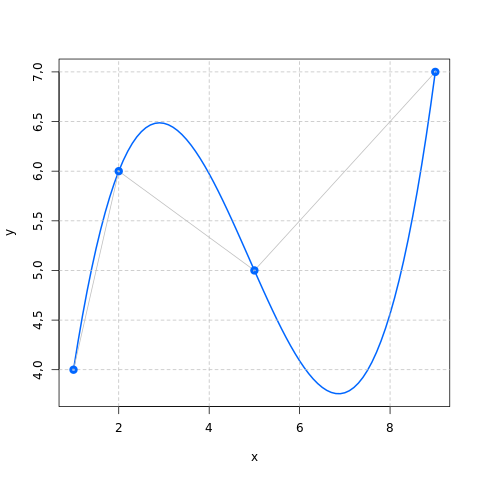
\includegraphics[width=0.75\textwidth]{interpolated.png}
	\caption{Исходные точки и график интерполяционного полинома}
	\label{fig:interpolated}
\end{figure}

%%%%%%%%%%%%%%%%%%%%%%%%%%%%%%%%%%%%%%%%

\clearpage

\section{\MakeUppercase{Заключение}}

В ходе выполнения лабораторно-практичес\-кой работы мы написали и~отладили код для вычисления полинома Лагранжа, затем с~его помощью интерполировали выбранные точки исходной функции $f(x)$ и построили график.

\end{document}
